\section{PDFBox}

\begin{frame}{PDFBox}
  	\begin{block}{visionneuse}
  		 \begin{itemize}
	   		\item visualiser cours
              		\item upload zip contenant les diapositives (format image)
	 	\end{itemize}
  	\end{block}

	Question: comment convertir un pdf en image?

	\begin{block}{Première approche}
  		\begin{itemize}
      			\item parser un pdf
      			\item jpedal
      			\item iText
  		\end{itemize}
	\end{block}
\end{frame}

\begin{frame}{PDFBox}
	\begin{block}{présentation}
		\begin{itemize}
			\item Projet open source (Apache Software Foundation)
			\item Java 
			\item Conversion pdf -$>$ image
			\item Limitation: police arial!
		\end{itemize}
	\end{block}

	\begin{block}{problèmes}
		\begin{itemize}
			\item redimensionnement
			\item décalage
			\item mauvais caractères imprimés
		\end{itemize}
	\end{block}
\end{frame}

\begin{frame}{problème: cropbox/mediabox}
	\begin{block}{redimensionnement}
		\begin{figure}[h]
        		\begin{center}
         		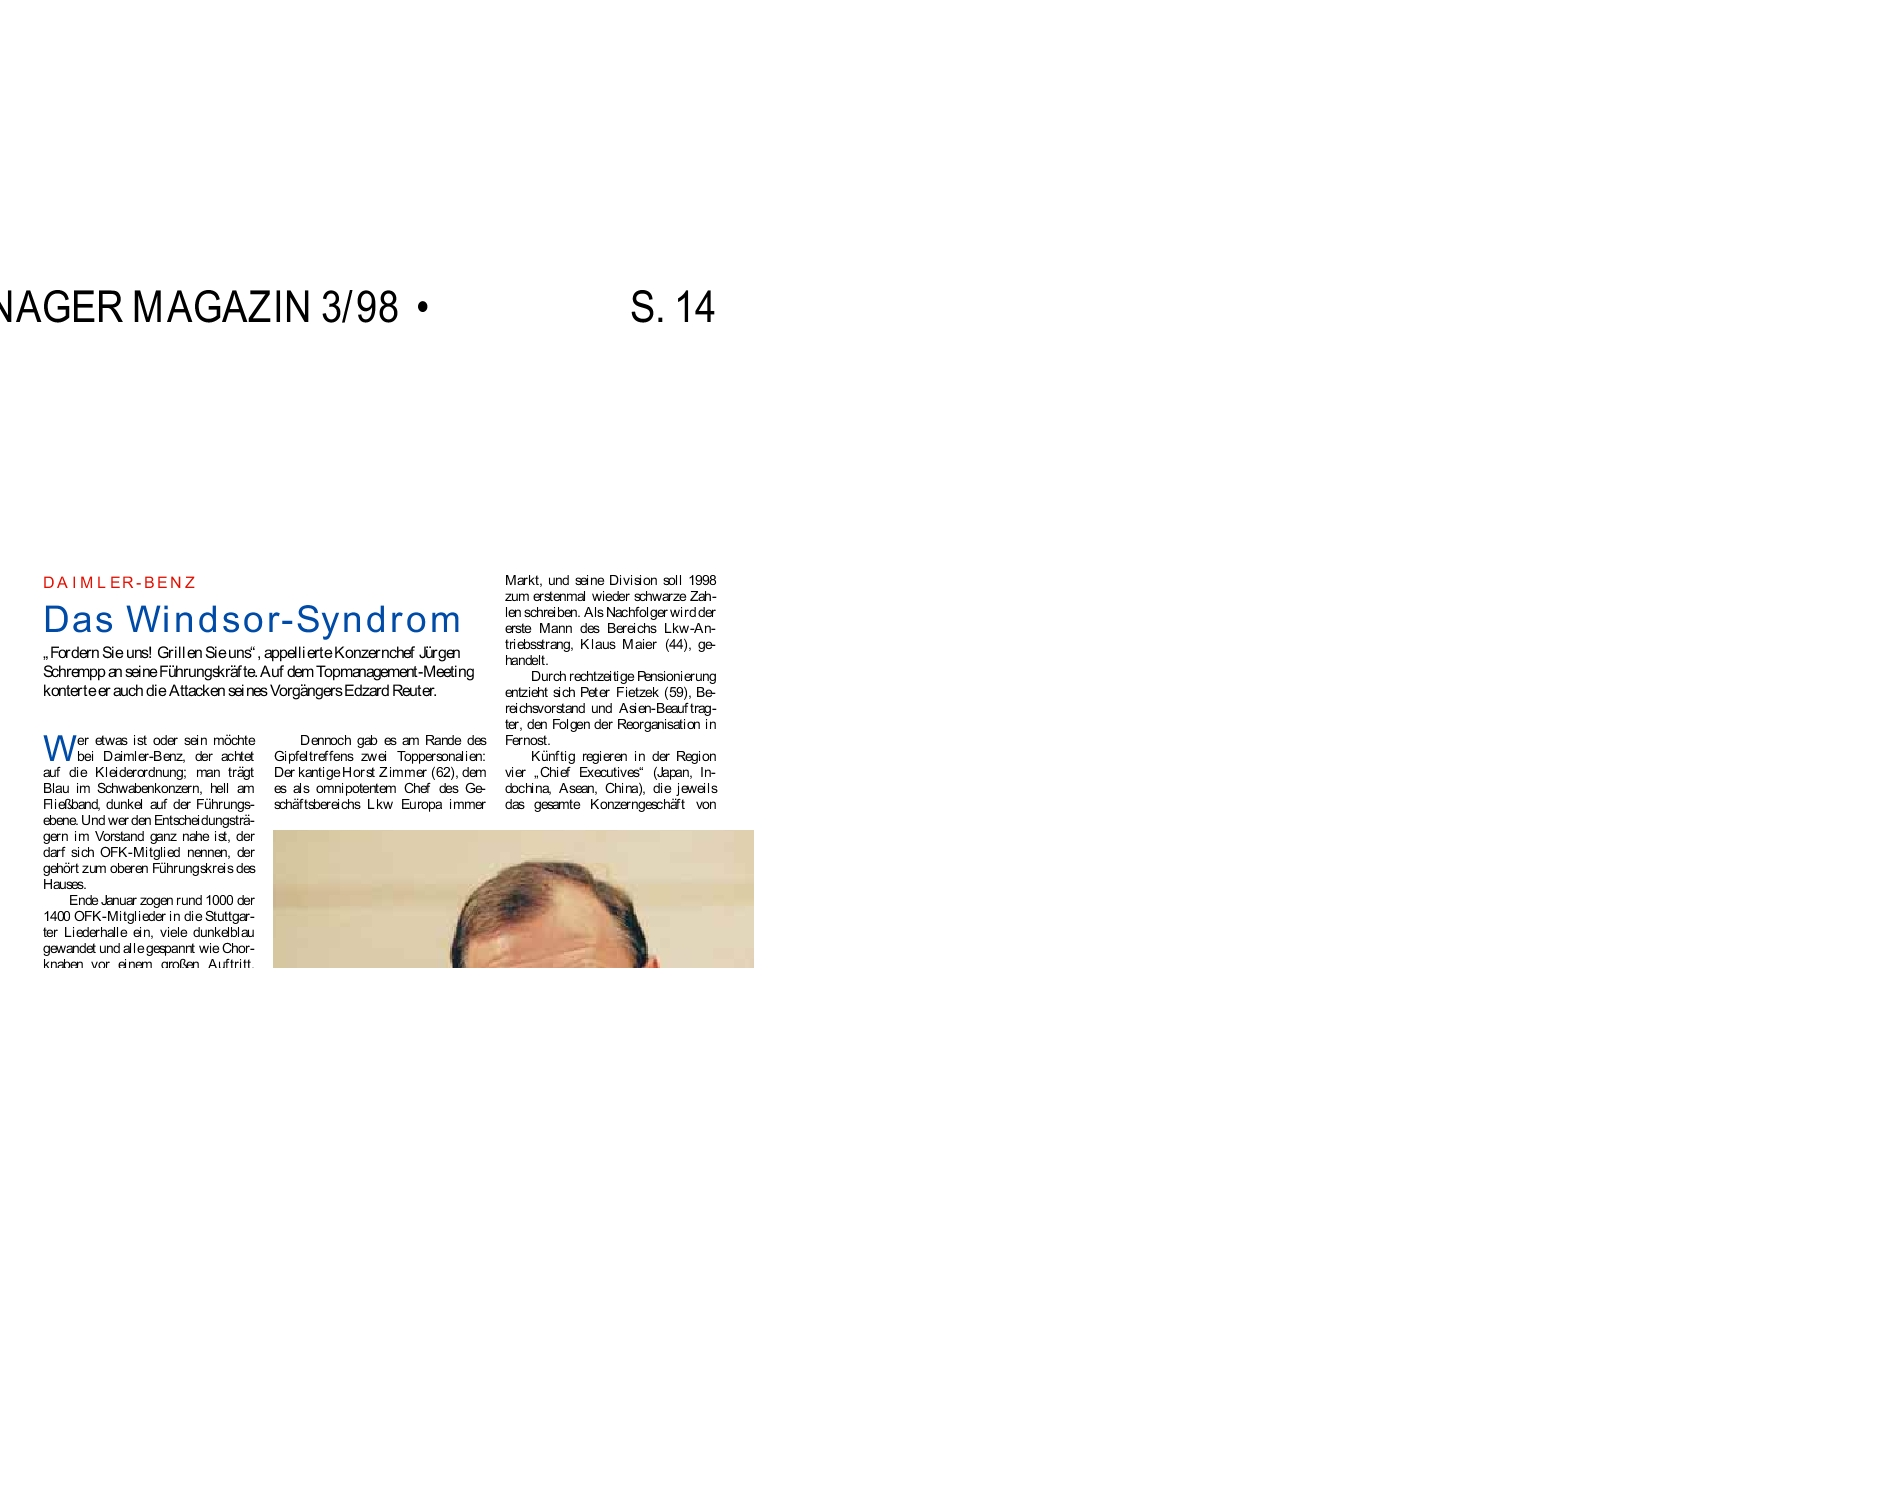
\includegraphics[scale=0.08]{images/fail1.jpg} 
        		\end{center}
        		\caption{erreur}
        		\label{erreur}
    		\end{figure}
	\end{block}
\end{frame}

\begin{frame}{Polices}
	\begin{block}{mauvais gestion des polices}
		\begin{figure}[h]
        		\begin{center}
         		
\includegraphics[scale=0.17]{images/fail2.jpg} 
        		\end{center}
        		\caption{erreur}
        		\label{erreur}
    		\end{figure}
	\end{block}
\end{frame}

%\begin{frame}{}
%	
%\end{frame}

